\chapter{Momentum}

Let's say a 2 kg block of putty is flying through space at 5 meters
per second, and it collides with a larger 3 kg block of putty that is not
moving at all. When the two blocks deform and stick to each other, how
fast will the resultant big block be moving?
\begin{center}
  
  \includegraphics[width=0.4\textwidth]{putty1.png}
  \includegraphics[width=0.4\textwidth]{putty2.png}
\end{center}
\index{momentum}


\begin{mdframed}[style=important, frametitle={Formula for Momentum}]
Every object has \newterm{momentum}. The momentum is a vector
quantity --- it points in the direction that the object is moving and has
a magnitude equal to its mass times its speed.
\begin{equation}
  p=mv
\end{equation}
\end{mdframed}

Given a set of objects that are interacting, we can sum all their
momentum vectors to get the total momenta. In such a set, the total
momentum will stay constant.
\begin{equation}
p = p_1 + p_2 + \dots + p_n = m_1v_1+m_2v_2 + \dots + m_nv_n
\end{equation}

In our example, one object has a momentum vector of magnitude of
10 kg m/s, the other has a momentum of magnitude 0.  Once they have
merged, they have a combined mass of 5 kg.  This means the velocity vector
must have magnitude 2 m/s and pointing in the same direction that the
first mass was moving.
\index{momentum!conservation of}
\begin{mdframed}[style=important, frametitle={Conservation of Momentum}]
\textbf{The total momentum of a system remains constant as long as no external forces act on it.}
In a collision or interaction, the momentum before the event must equal the momentum after the event:
\begin{equation}
p_{\text{initial}} = p_{\text{final}}
\end{equation}
This applies whether the collision is elastic, inelastic, or perfectly inelastic. Even if kinetic energy is lost (as heat, sound, or deformation), momentum is still conserved because it depends only on mass and velocity, not on energy.
\end{mdframed}

\begin{Exercise}[title={Cars on Ice}, label=cars_on_ice]
A car weighing 1000 kg is going north at 12 m/s.  Another car weighing
1500 kg is going east at 16 m/s.  They both hit a patch of ice (with
zero friction) and collide.  Steel is bent, and the two objects become
one.  How what is the velocity vector (direction and magnitude) of the
new object sliding across the ice?
\includegraphics[width=0.4\textwidth]{icecar.png}
\includegraphics[width=0.4\textwidth]{icecar2.png}

\end{Exercise}
\begin{Answer}[ref=cars_on_ice]
  The momentum of the first car is 12,000 kg m/s in the north direction.

  The momentum of the second car is 24,000 kg m/s in the east direction.

  The new object will be moving northeast. What is the angle compared with the east?

  $$\theta = \arctan{\frac{12,000}{24,000}} \approx 0.4636 \text{ radians } \approx 26.565\text{ degrees north of east}$$

  The magnitude of the momentum of the new object is $\sqrt{12,000^2 + 24,000^2} \approx 26,833\text{ kg m/s}$

  Its new mass is 2,5000 kg.  So the speed will be $26,833/2,500 = 10.73$ m/s.
\end{Answer}


Note that kinetic energy ($1/2 m v^2$) is \emph{not} conserved
here.  Before the collision, the moving putty block has $(1/2)(2)(5^2) = 25$
joules of kinetic energy.  Afterward, the big block has $(1/2)(5)(2^2)
= 10$ joules of kinetic energy.  What happened to the energy that was
lost? It was used up deforming the putty.

What if the blocks were marble instead of putty?  Then there would be
very little deforming, so kinetic energy \emph{and} momentum would be
conserved. The two blocks would end up having different velocity
vectors.

Let's assume for a moment that they strike each other straight on, so
there is motion in only one direction, both before and after the
collision.  Can we solve for the speeds of the first block ($v_1$) and
the second block ($v_2$)?

We end up with two equations. Conservation of momentum says:

$$2 v_1 + 3 v_2 = 10$$

Conservation of kinetic energy says:

$$(1/2)(2)(v_1^2) + (1/2)(3)(v_2^2) = 25$$

Using the first equation, we can solve for $v_1$ in terms of $v_2$:

$$v_1 = \frac{10 - 3 v_2}{2}$$

Substituting this into the second equation, we get:

$$\left(\frac{10 - 3 v_2}{2}\right)^2 + \frac{3 v_2^2}{2} = 25$$

Simplifying, we get:

$$v_2^2 - 4 v_2 + 0 = 0$$

This quadratic has two solutions: $v_2 = 0$ and $v_2 = 4$.  $v_2 = 0$
represents the situation before the collision.  Substituting in $v_2 = 4$:

$$v_1 = \frac{10 - 3(4)}{2} = -1$$

Thus, if the blocks are hard enough that kinetic energy is conserved,
after the collision, the smaller block will be heading in the opposite
direction at 1 m/s. The larger block will be moving at 4 m/s in the
direction of the original motion.

\begin{Exercise}[title={Billiard Balls}, label=billiards]
  
A billiard ball weighing 0.4 kg and traveling at 3 m/s hits a billiard
ball (same weight) at rest. It strikes obliquely (neither perpendicular nor parallel), so that the ball at rest starts to
move at a 45 degree angle from the path of the ball that hit it.

Assuming all kinetic energy is conserved, what is the velocity
vector of each ball after the collision?

\includegraphics[width=.75\textwidth]{poolball.png}

\end{Exercise}
\begin{Answer}[ref=billiards]

  The original forward momentum was 1.2 kg m/s.  The original kinetic energy is $(1/2)(0.4)(3^2)$ = 1.8 joules. 

  Let $s$ be the post-collision speed of the ball that had been at
  rest.  Let $x$ and $y$ be the forward and sideways speeds
  (post-collision) of the other ball. Conservation of kinetic energy says

  $$(1/2)(0.4)(s^2) + (1/2)(0.4)(x^2+y^2) = 1.8$$

  Forward momentum is conserved:

  $$0.4\frac{s}{\sqrt{2}} + 0.4 x = 1.2$$

  Which can be rewritten:

  $$x = 3 - \frac{s}{\sqrt{2}}$$
  
  Sideways momentum stays zero:

  $$(0.4)\frac{s}{\sqrt{2}} - 0.4 y = 0.0$$

  Which can be rewritten:

  $$y = \frac{s}{\sqrt{2}}$$

  Substituting into to the conservation of kinetic energy equation above:

  $$(1/2)(0.4)(s^2) + (1/2)(0.4)(\left(3 - \frac{s}{\sqrt{2}}\right)^2+\left(\frac{s}{\sqrt{2}}\right)^2 = 1.8$$

  Which can be rewritten:

  $$s^2 - \frac{3}{\sqrt{2}} s + 0 = 0$$

  There are two solutions to this quadratic: $s = 0$ (before collision) and $s = \frac{3}{\sqrt{2}}$. Thus,

  $$y = \frac{3}{2}$$

  and

  $$x = 3 - \frac{3}{2} = \frac{3}{2}$$

  So, both balls careen off at $45^\circ$ angles at the exact same speed. 

  
\end{Answer}
\section{Impulse}
We can talk about a \emph{change in Momentum} as what we refer to as \newterm{Impulse}. When an object has a change in momentum, it is said to have been given an Impulse. Since momentum is a vector quantity, impulse is as well. 

\begin{mdframed}[style=important, frametitle={Formula for Impulse}]
Impulse, $\textbf{J}$ said to be the change in momentum, is given by:
\begin{equation}
  \textbf{J} = \Delta p
\end{equation}
Equivallently, it can be given as the following equation, in terms of force:
\begin{equation}
  \textbf{J} = F\Delta t \label{eq:impulse-momentum1}
\end{equation}
If the force varies with time, we use integration to find the impulse:
\begin{equation}
  \textbf{J} = \int_{t_0}^{t_1} F(t) dt \label{eq:impulse-momentum2}
\end{equation}
Both Equations~\eqref{eq:impulse-momentum1} and \eqref{eq:impulse-momentum2} are referred to as the \textbf{Impulse-Momentum Theorem}. 
\end{mdframed}
By the impulse momentum theorem, a large force for a short time \textit{or} a small force for a long time can produce the same impulse.

\subsection{Golf Swings}
The best example of impulse in action is a golf swing. Let's analyse this using equations:

The force of your swing will theoretically always be the same, as the maximum force you can apply is limited by human ability. You cannot change the human-provided force, however, you can increase the \emph{contact time} of your club on the ball.
\[
\textbf{J} = F\Delta t
\]

Since $\text{J}$ is equivalent to $\Delta p$, $\Delta t$, the contact time of the swing, has a proportional relationship with the momentum of the ball, which starts of as $0$. Thus, it can be said:
\[
\Delta p \propto \Delta t
\]
And, holding $F$, $m$, and assuming the golf ball is initially at rest, $p_i=0$, we can say
\[
v_f \propto \Delta t
\]

So the longer the contact time of a golf swing (or any swing-based sport, really), the greater the velocity.
\section{Collisions}
\index{collisions}
When two (or more) objects collide, we can classify their collision as one of three main categories. These classifications tell us when we can apply the conservation of momentum, the consevation of kinetic energy, both, or neither. Momentum is only conserved when the system is isolated, meaning no external forces act on the system.

\subsection{Elastic Collision}
Recall our billiard ball problem from Exercise~\ref{billiards}. That problem provides both balls with velocity after the collision. In an ideal and more realistic billiards scenario, one ball transfers all of its velocity onto the other ball (in this case, the red ball stops and the blue continues with close to same velocity that the red ball had initially), as seen in Figure~\ref{fig:billiardElasticCollision} This would be a \newterm{elastic collision}\index{collisions!elastic}. 

In an elastic collision, \emph{both momentum and kinetic energy are conserved}. There is minimal to zero loss of energy in the collision. Although no collision is ever \emph{truly} elastic (due to existing but miminmal deformation of objects, sound, a transfer of heat through molecular changes, etc), we can think of a collision like this as perfectly elastic. The sound of billiard balls colliding is obsolete (especially compared to a car crash), so very little energy is lost to sound. 

\begin{figure}[H] % FIGURE made with matcha.io
    \centering




\tikzset{every picture/.style={line width=0.75pt}} %set default line width to 0.75pt        

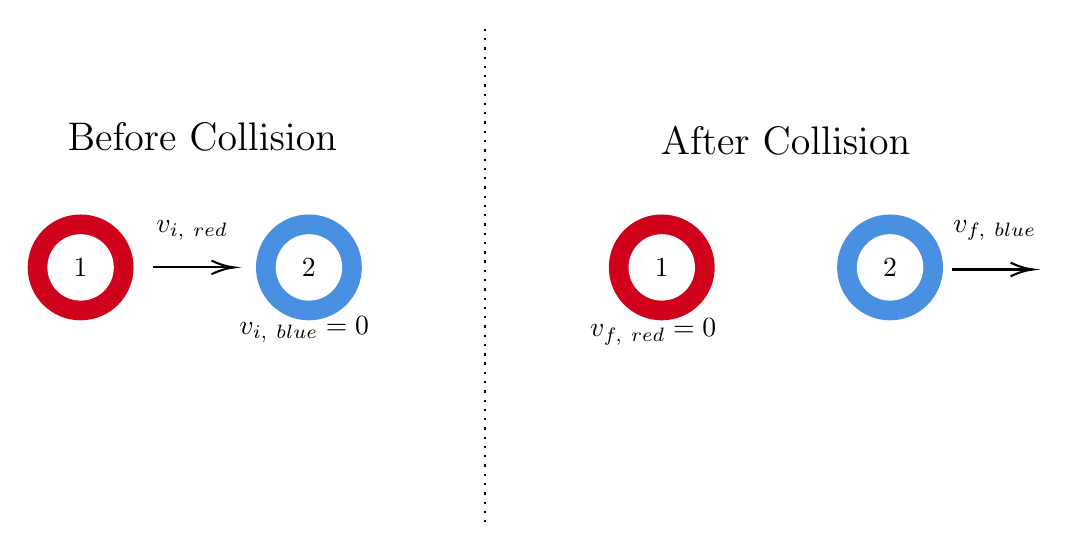
\begin{tikzpicture}[x=0.75pt,y=0.75pt,yscale=-1,xscale=1]
%uncomment if require: \path (0,200); %set diagram left start at 0, and has height of 200

%Shape: Circle [id:dp008663425032839123] 
\draw  [color={rgb, 255:red, 208; green, 2; blue, 27 }  ,draw opacity=1 ][fill={rgb, 255:red, 208; green, 2; blue, 27 }  ,fill opacity=1 ] (7,87) .. controls (7,73.19) and (18.19,62) .. (32,62) .. controls (45.81,62) and (57,73.19) .. (57,87) .. controls (57,100.81) and (45.81,112) .. (32,112) .. controls (18.19,112) and (7,100.81) .. (7,87) -- cycle ;
%Shape: Circle [id:dp9535962022773641] 
\draw  [color={rgb, 255:red, 74; green, 144; blue, 226 }  ,draw opacity=1 ][fill={rgb, 255:red, 74; green, 144; blue, 226 }  ,fill opacity=1 ] (117,87) .. controls (117,73.19) and (128.19,62) .. (142,62) .. controls (155.81,62) and (167,73.19) .. (167,87) .. controls (167,100.81) and (155.81,112) .. (142,112) .. controls (128.19,112) and (117,100.81) .. (117,87) -- cycle ;
%Straight Lines [id:da7947804457183854] 
\draw [color={rgb, 255:red, 0; green, 0; blue, 0 }  ,draw opacity=1 ]   (67,87) -- (104,87) ;
\draw [shift={(106,87)}, rotate = 180] [color={rgb, 255:red, 0; green, 0; blue, 0 }  ,draw opacity=1 ][line width=0.75]    (10.93,-3.29) .. controls (6.95,-1.4) and (3.31,-0.3) .. (0,0) .. controls (3.31,0.3) and (6.95,1.4) .. (10.93,3.29)   ;
%Shape: Circle [id:dp3473081297928793] 
\draw  [color={rgb, 255:red, 208; green, 2; blue, 27 }  ,draw opacity=1 ][fill={rgb, 255:red, 208; green, 2; blue, 27 }  ,fill opacity=1 ] (287,87) .. controls (287,73.19) and (298.19,62) .. (312,62) .. controls (325.81,62) and (337,73.19) .. (337,87) .. controls (337,100.81) and (325.81,112) .. (312,112) .. controls (298.19,112) and (287,100.81) .. (287,87) -- cycle ;
%Shape: Circle [id:dp2823305825418243] 
\draw  [color={rgb, 255:red, 74; green, 144; blue, 226 }  ,draw opacity=1 ][fill={rgb, 255:red, 74; green, 144; blue, 226 }  ,fill opacity=1 ] (397,87) .. controls (397,73.19) and (408.19,62) .. (422,62) .. controls (435.81,62) and (447,73.19) .. (447,87) .. controls (447,100.81) and (435.81,112) .. (422,112) .. controls (408.19,112) and (397,100.81) .. (397,87) -- cycle ;
%Straight Lines [id:da6314481364721517] 
\draw [color={rgb, 255:red, 0; green, 0; blue, 0 }  ,draw opacity=1 ]   (452,88) -- (489,88) ;
\draw [shift={(491,88)}, rotate = 180] [color={rgb, 255:red, 0; green, 0; blue, 0 }  ,draw opacity=1 ][line width=0.75]    (10.93,-3.29) .. controls (6.95,-1.4) and (3.31,-0.3) .. (0,0) .. controls (3.31,0.3) and (6.95,1.4) .. (10.93,3.29)   ;
%Shape: Circle [id:dp06335952269010947] 
\draw  [color={rgb, 255:red, 255; green, 255; blue, 255 }  ,draw opacity=1 ][fill={rgb, 255:red, 255; green, 255; blue, 255 }  ,fill opacity=1 ] (16.5,87) .. controls (16.5,78.44) and (23.44,71.5) .. (32,71.5) .. controls (40.56,71.5) and (47.5,78.44) .. (47.5,87) .. controls (47.5,95.56) and (40.56,102.5) .. (32,102.5) .. controls (23.44,102.5) and (16.5,95.56) .. (16.5,87) -- cycle ;
%Shape: Circle [id:dp964345354843358] 
\draw  [color={rgb, 255:red, 255; green, 255; blue, 255 }  ,draw opacity=1 ][fill={rgb, 255:red, 255; green, 255; blue, 255 }  ,fill opacity=1 ] (126.5,87) .. controls (126.5,78.44) and (133.44,71.5) .. (142,71.5) .. controls (150.56,71.5) and (157.5,78.44) .. (157.5,87) .. controls (157.5,95.56) and (150.56,102.5) .. (142,102.5) .. controls (133.44,102.5) and (126.5,95.56) .. (126.5,87) -- cycle ;
%Shape: Circle [id:dp9487777680881678] 
\draw  [color={rgb, 255:red, 255; green, 255; blue, 255 }  ,draw opacity=1 ][fill={rgb, 255:red, 255; green, 255; blue, 255 }  ,fill opacity=1 ] (296.5,87) .. controls (296.5,78.44) and (303.44,71.5) .. (312,71.5) .. controls (320.56,71.5) and (327.5,78.44) .. (327.5,87) .. controls (327.5,95.56) and (320.56,102.5) .. (312,102.5) .. controls (303.44,102.5) and (296.5,95.56) .. (296.5,87) -- cycle ;
%Shape: Circle [id:dp38208952626529435] 
\draw  [color={rgb, 255:red, 255; green, 255; blue, 255 }  ,draw opacity=1 ][fill={rgb, 255:red, 255; green, 255; blue, 255 }  ,fill opacity=1 ] (406.5,87) .. controls (406.5,78.44) and (413.44,71.5) .. (422,71.5) .. controls (430.56,71.5) and (437.5,78.44) .. (437.5,87) .. controls (437.5,95.56) and (430.56,102.5) .. (422,102.5) .. controls (413.44,102.5) and (406.5,95.56) .. (406.5,87) -- cycle ;
%Straight Lines [id:da09270525196159507] 
\draw [line width=0.75]  [dash pattern={on 0.84pt off 2.51pt}]  (227,-28) -- (227,213) ;

% Text Node
\draw (67,63) node [anchor=north west][inner sep=0.75pt]   [align=left] {$\displaystyle v_{i,\ red}$};
% Text Node
\draw (90.64,24.12) node   [align=left] {{\Large Before Collision}};
% Text Node
\draw (107,109.4) node [anchor=north west][inner sep=0.75pt]    {$v_{i,\ blue} =0$};
% Text Node
\draw (371.63,26.12) node   [align=left] {{\Large After Collision}};
% Text Node
\draw (451,63) node [anchor=north west][inner sep=0.75pt]   [align=left] {$\displaystyle v_{f,\ blue}$};
% Text Node
\draw (276,110.4) node [anchor=north west][inner sep=0.75pt]    {$v_{f,\ red} =0$};
% Text Node
\draw (312,87) node    {$1$};
% Text Node
\draw (32,87) node    {$1$};
% Text Node
\draw (142,87) node    {$2$};
% Text Node
\draw (422,87) node    {$2$};


\end{tikzpicture}
    \caption{Example of an elastic biliard collision.}
    \label{fig:billiardElasticCollision}
\end{figure}

Another example to consider here is Newton's Cradle. There are two videos demonstrating momentum in Newton's Cradle on your digital resources. % possible diagram for this?

In equation format, Elastic Collisions are represented by the sums of momentum and kinetic energy before and after the collision being equal:
\[\text{total }\textbf{p}_{\text{before collision}} = \text{total }\textbf{p}_{\text{after collision}} \implies m_1v_{i,1} + m_2v_{i,2} + \cdots  = m_1v_{f,1} + m_2v_{f,2} + \cdots\]
\emph{and}
\[\text{total }\textbf{KE}_{\text{before collision}} = \text{total }\textbf{KE}_{\text{after collision}}\]

\subsection{Inelastic Collisions}
Inelastic collisions, then, are ones in which the total kinetic energy after the collision is \emph{different} than before the collision, in other words, there is a change in kinetic energy, usually lost due to friction, heat, or deformation. 

However, momentum \emph{is} conserved, meaning we can apply conservation of momentum principles.

\[\text{total }\textbf{p}_{\text{before collision}} = \text{total }\textbf{p}_{\text{after collision}} \implies m_1v_{i,1} + m_2v_{i,2} + \cdots  = m_1v_{f,1} + m_2v_{f,2} + \cdots\]

A good example of an elastic collision is dropping a basketball on a floor from an initial height. It will never return to its initial height after ``colliding'' with the floor, as kinetic energy is `lost' to sound and deformation of the ball. The missing height can be equated to the lost energy. See Figure~\ref{fig:basketballInelastic}

\begin{figure}[H]
    \centering
    

% Gradient Info
  
\tikzset {_ow2fjvq0g/.code = {\pgfsetadditionalshadetransform{ \pgftransformshift{\pgfpoint{89.1 bp } { -108.9 bp }  }  \pgftransformscale{1.32 }  }}}
\pgfdeclareradialshading{_rpiy6ip9a}{\pgfpoint{-72bp}{88bp}}{rgb(0bp)=(1,1,1);
rgb(0bp)=(1,1,1);
rgb(25bp)=(0,0,0);
rgb(400bp)=(0,0,0)}

% Gradient Info
  
\tikzset {_twget7vfx/.code = {\pgfsetadditionalshadetransform{ \pgftransformshift{\pgfpoint{89.1 bp } { -108.9 bp }  }  \pgftransformscale{1.32 }  }}}
\pgfdeclareradialshading{_4fv2or85u}{\pgfpoint{-72bp}{88bp}}{rgb(0bp)=(1,1,1);
rgb(0bp)=(1,1,1);
rgb(25bp)=(0,0,0);
rgb(400bp)=(0,0,0)}
\tikzset{every picture/.style={line width=0.75pt}} %set default line width to 0.75pt        

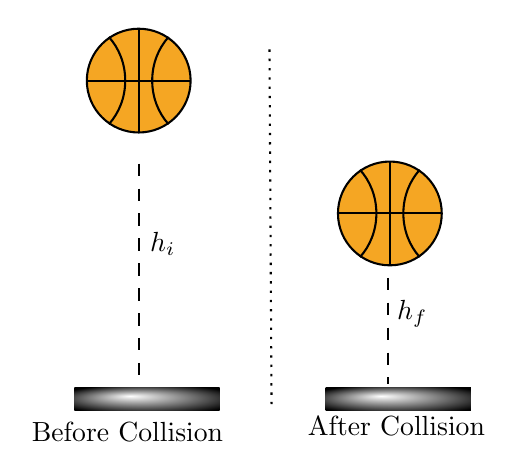
\begin{tikzpicture}[x=0.75pt,y=0.75pt,yscale=-1,xscale=1]
%uncomment if require: \path (0,224); %set diagram left start at 0, and has height of 224

%Shape: Circle [id:dp31951467519732246] 
\draw  [fill={rgb, 255:red, 245; green, 166; blue, 35 }  ,fill opacity=1 ] (46,39) .. controls (46,25.19) and (57.19,14) .. (71,14) .. controls (84.81,14) and (96,25.19) .. (96,39) .. controls (96,52.81) and (84.81,64) .. (71,64) .. controls (57.19,64) and (46,52.81) .. (46,39) -- cycle ;
%Straight Lines [id:da9792388690408605] 
\draw    (71,14) -- (71,64) ;
%Straight Lines [id:da9432518901820793] 
\draw    (46,39) -- (96,39) ;
%Shape: Arc [id:dp6381408760983348] 
\draw  [draw opacity=0] (56.61,17.97) .. controls (61.49,23.38) and (64.5,30.81) .. (64.5,39) .. controls (64.5,47.19) and (61.49,54.62) .. (56.61,60.03) -- (37,39) -- cycle ; \draw   (56.61,17.97) .. controls (61.49,23.38) and (64.5,30.81) .. (64.5,39) .. controls (64.5,47.19) and (61.49,54.62) .. (56.61,60.03) ;  
%Shape: Arc [id:dp18945185949635923] 
\draw  [draw opacity=0] (85.39,60.03) .. controls (80.51,54.62) and (77.5,47.19) .. (77.5,39) .. controls (77.5,30.81) and (80.51,23.38) .. (85.39,17.97) -- (105,39) -- cycle ; \draw   (85.39,60.03) .. controls (80.51,54.62) and (77.5,47.19) .. (77.5,39) .. controls (77.5,30.81) and (80.51,23.38) .. (85.39,17.97) ;  

%Straight Lines [id:da3244593608524523] 
\draw  [dash pattern={on 4.5pt off 4.5pt}]  (71,79) -- (71,181) ;
%Shape: Rectangle [id:dp30204448918965] 
\draw  [draw opacity=0][shading=_rpiy6ip9a,_ow2fjvq0g] (40,187) -- (110,187) -- (110,198) -- (40,198) -- cycle ;
%Shape: Circle [id:dp9684977004197513] 
\draw  [fill={rgb, 255:red, 245; green, 166; blue, 35 }  ,fill opacity=1 ] (167,103) .. controls (167,89.19) and (178.19,78) .. (192,78) .. controls (205.81,78) and (217,89.19) .. (217,103) .. controls (217,116.81) and (205.81,128) .. (192,128) .. controls (178.19,128) and (167,116.81) .. (167,103) -- cycle ;
%Straight Lines [id:da09155876575740851] 
\draw    (192,78) -- (192,128) ;
%Straight Lines [id:da5376981986809476] 
\draw    (167,103) -- (217,103) ;
%Shape: Arc [id:dp21961184168827608] 
\draw  [draw opacity=0] (177.61,81.97) .. controls (182.49,87.38) and (185.5,94.81) .. (185.5,103) .. controls (185.5,111.19) and (182.49,118.62) .. (177.61,124.03) -- (158,103) -- cycle ; \draw   (177.61,81.97) .. controls (182.49,87.38) and (185.5,94.81) .. (185.5,103) .. controls (185.5,111.19) and (182.49,118.62) .. (177.61,124.03) ;  
%Shape: Arc [id:dp8628176960613382] 
\draw  [draw opacity=0] (206.39,124.03) .. controls (201.51,118.62) and (198.5,111.19) .. (198.5,103) .. controls (198.5,94.81) and (201.51,87.38) .. (206.39,81.97) -- (226,103) -- cycle ; \draw   (206.39,124.03) .. controls (201.51,118.62) and (198.5,111.19) .. (198.5,103) .. controls (198.5,94.81) and (201.51,87.38) .. (206.39,81.97) ;  

%Straight Lines [id:da2940374184344693] 
\draw  [dash pattern={on 4.5pt off 4.5pt}]  (191,134) -- (191,185) ;
%Shape: Rectangle [id:dp15122863084219784] 
\draw  [draw opacity=0][shading=_4fv2or85u,_twget7vfx] (161,187) -- (231,187) -- (231,198) -- (161,198) -- cycle ;

%Straight Lines [id:da6359048401622878] 
\draw  [dash pattern={on 0.84pt off 2.51pt}]  (134,24) -- (135,196) ;

% Text Node
\draw (75,110.4) node [anchor=north west][inner sep=0.75pt]    {$h_{i}$};
% Text Node
\draw (18,202) node [anchor=north west][inner sep=0.75pt]   [align=left] {Before Collision};
% Text Node
\draw (194,143.4) node [anchor=north west][inner sep=0.75pt]    {$h_{f}$};
% Text Node
\draw (151,199) node [anchor=north west][inner sep=0.75pt]   [align=left] {After Collision};


\end{tikzpicture}
    \caption{An example of a (partially) inelastic collision between the floor and a basketball.}
    \label{fig:basketballInelastic}
\end{figure}

\subsection{Perfectly Inelastic}
A collision is \emph{perfectly inelastic} when the masses stick together after the collision.\index{collisions!perfectly inelastic}In this kind of collision, the \emph{maximum} kinetic energy is lost (crumpling, bending, embedding of objects) and share the same final velocity. 

The most common example of a perfectly inelastic collision is a car crash, especially high speed T-Bones. In this case, a car at a high speed collides with a car at a lower speed, resulting in a combined final speed as the cars interact on a molecular level and a large portion of energy is lost.


\begin{Exercise}[title={Two Carts}, label=carts_elastic]
Two carts on a frictionless track collide elastically.

Cart A has mass $2.0$ kg and is moving to the right at $3.0$ m/s.

Cart B has mass $1.0$ kg and is initially at rest.

They collide head-on elastically.

Find the final velocities of both carts. Hint: You may have to do a few equation substitutions
\end{Exercise}

\begin{Answer}[ref=carts_elastic]
Because both carts collide elastically, the Conservation of Kinetic Energy and Conservation of Momentum both apply.

We can rearrange the Conservation of Kinetic Energy in the following ways:
\begin{align*}
\frac{1}{2}m_1 v_{1i}^2 + \frac{1}{2}m_2 v_{2i}^2&=\frac{1}{2}m_1 v_{1f}^2 + \frac{1}{2}m_2 v_{2f}^2 \\ 
\frac{1}{2}m_1 v_{1i}^2 + \frac{1}{2}m_2 v_{2i}^2 - \frac{1}{2}m_1 v_{1f}^2 - \frac{1}{2}m_2 v_{2f}^2 &= 0\\ 
m_1 v_{1i}^2 + m_2 v_{2i}^2 - m_1 v_{1f}^2 - m_2 v_{2f}^2 &= 0\\ 
m_1 v_{1i}^2 - m_1 v_{1f}^2 + m_2 v_{2i}^2 - m_2 v_{2f}^2 &= 0 \\ 
m_1 (v_{1i}^2 - v_{1f}^2) + m_2 (v_{2i}^2 -  v_{2f}^2) &= 0 \\ 
m_1 (v_{1i} - v_{1f})(v_{1i} + v_{1f})+m_2 (v_{2i} - v_{2f})(v_{2i} + v_{2f}) &= 0 \tag{1}\label{eq:1}\\
\end{align*}

And rearranging Conservation of Momentum:
\begin{align*}
  m_1 v_{1i} + m_2 v_{2i} &= m_1 v_{1f} + m_2 v_{2f} \\
  m_1 v_{1i} + m_2 v_{2i} - m_1 v_{1f} - m_2 v_{2f} &= 0\\
  m_1 (v_{1i} - v_{1f}) + m_2 (v_{2i} - v_{2f}) &= 0 \\
  m_1 (v_{1i} - v_{1f}) &= -m_2 (v_{2i} - v_{2f}) \tag{2}\label{eq:2}\\
\end{align*}

Inputting Equation~\ref{eq:2} into Equation~\label{eq:1}:

\begin{align*}
m_1 (v_{1i} - v_{1f})(v_{1i} + v_{1f})+m_2 (v_{2i} - v_{2f})(v_{2i} + v_{2f}) &= 0 \\
- m_2 (v_{2i} - v_{2f})(v_{1i} + v_{1f})+m_2 (v_{2i} - v_{2f})(v_{2i} + v_{2f}) &= 0 \\ 
m_2 (v_{2i} - v_{2f})\left[\, (v_{2i} + v_{2f}) - (v_{1i} + v_{1f}) \right] &= 0 \\ 
(v_{2i} + v_{2f}) - (v_{1i} + v_{1f}) &= 0 \hfill \text{ assuming } v_{2i} \ne v_{2f}\\
v_{2f} - v_{1f} &= v_{1i} - v_{2i} \tag{3}\\ 
\end{align*}
Equation 3 tells us that, in an elastic collision, the relative speed of separation is equal to relative speed of approach. 
This allows us to do the following plug-ins:
\begin{align*}
m_1 v_{1i} + m_2 v_{2i}&=m_1 v_{1f}+m_2 (v_{1f} + v_{1i} - v_{2i}) \\ 
m_1 v_{1i} + m_2 v_{2i}&=(m_1 + m_2) v_{1f} + m_2 v_{1i} - m_2 v_{2i} \\
(m_1 - m_2) v_{1i} + 2 m_2 v_{2i}&=(m_1 + m_2)\, v_{1f} \\ 
v_{1f}&=\frac{m_1 - m_2}{m_1 + m_2} v_{1i}+\frac{2m_2}{m_1 + m_2} v_{2i} \label{eq:vel1Final}\\
\end{align*}
The same process results in $v_{2f}$:

\begin{equation}
  v_{2f} =\frac{2m_1}{m_1 + m_2} v_{1i}+\frac{m_2 - m_1}{m_1 + m_2} v_{2i}\label{eq:vel2Final}
\end{equation}

Equations~\ref{eq:vel1Final} and \ref{eq:vel2Final} can be very useful but take a while to derive. Make sure you understand the process to solve for them. Let's plug in the values:
$$v_{1f} = \frac{2 - 1}{2 + 1}(3.0)
= \frac{1}{3}(3.0)
= 1.0\text{ m/s}$$
$$v_{2f} = \frac{2(2)}{2+1}(3.0)
= \frac{4}{3}(3.0)
= 4.0\text{ m/s}$$
\end{Answer}

\begin{Exercise}[title={Car Crash}, label={car_crash}]
Sometimes, car companies will intentionally crash cars in order to test the safety of their prototypes.

Two cars collide head-on on a straight, frictionless test track, where east is considered positive.

Car A has mass $1000$ kg and is traveling \emph{east} at $20$ m/s. Car B has mass $1500$ kg and is traveling \emph{west} at $10$ m/s.

During the collision, the cars do not stick together. After the collision, Car A is observed to move east at $5$ m/s.

Find the final velocity of Car B. You are told kinetic energy is not conserved. Is this an elastic or inelastic collision?
\end{Exercise}

\begin{Answer}[ref={car_crash}]
Using the Conservation of Momentum theorem:
\begin{align*}
m_A v_{A,i} + m_B v_{B,i}&= m_A v_{A,f} + m_B v_{B,f} \\ 
(1000)(20) + (1500)(-10)&= (1000)(5) + (1500)v_{B,f} \\
20000 -15000 - 5000&= (1500)v_{B,f} \\
0&= (1500)v_{B,f} \\
v_{B,f} = 0 \text {m/s}\\
\end{align*}
The final velocity of Car B is $0$ m/s. The collision must be inelastic as both velocities change and kinetic energy is not conserved.
\end{Answer}

\begin{Exercise}[title={Ready, Aim, Fire!}, label=bullet_in_wood]
A $m_{bullet}=10$ g bullet is fired horizontally at $500$ m/s into a wooden block of mass $m_{block}=2.00$ kg resting on a frictionless horizontal surface. The bullet embeds itself in the block, such that a loud bang was heard and the \emph{block-bullet system} slides together after the collision.

\begin{enumerate}[label=(\alph*)]
  \item What is the velocity of the \emph{block-bullet system} after the collision?
  \item How much kinetic energy was lost in the collision?
  \item A collision is considered \textit{perfectly inelastic} if more than $95\%$ of the initial energy is lost. Classify the \emph{block-bullet system} collision by first finding the percent of energy lost.
\end{enumerate}
\end{Exercise}

\begin{Answer}[ref=bullet_in_wood]
\begin{enumerate}[label=(\alph*)]
  \item Using the conservation of momentum, we can say that:
  \begin{align*}
    m_{bullet}(v_{bullet}) + m_{block}(0) &= (m_{bullet} + m_{block})v_f \\ 
    (0.01)(500) + (2)(0) &= ((0.01) + (2))v_f \\ 
    v_f &= \frac{(500)(0.01)}{2.01} \\ 
    v_f &\approx 2.49 \text{m/s}
  \end{align*}
  The \emph{block-bullet system} moves at a speed of $2.49$ m/s, in the same direction the bullet was fired.
  \item 
  To find the initial kinetic energy, we use the initial velocity:
  \[KE_i = \frac{1}{2}(0.01)(500)^2 = 1250\]
  And, to find the final kinetic energy, we use the summed masses and the calculated final velocity
  \[KE_f = \frac{1}{2}(2.01)(2.49)^2 \approx 6.23\]
  So the net energy lost is the difference:
  $$\Delta KE = KE_i - KE_f \approx 1250 - 6.23 \approx 1243.7 \,\text{J}$$
  \item 
  $$\text{Fraction lost} = \frac{\Delta KE}{KE_i}= \frac{1243.7}{1250}\approx 0.99496$$
  So $99.5\%$ percent of the energy is lost. It is impossible for this to be an elastic collision, so this has to be an inelastic collision. Because \emph{more} than $95\%$ of the energy is lost, the collision is perfectly inelastic (by the problem guidelines).
\end{enumerate}
\end{Answer}

\section{Momentum, Center of Mass, and Explosions}

We have previously talked about finding the center of mass of an object (or objects). Now that we know about momentum, we can think about the center of mass in a different way.

Explosions typically involve an object breaking into pieces with internal forces (the forces of the explosion acting between fragments). The key is:

\textbf{Internal forces cannot change the motion of the center of mass.} This means that even during a violent explosion, the center of mass of the system continues moving exactly as it would if no explosion occurred. How does this work? It involves finding the sum of all momenta of the object.

\emph{Before and after the explosion:}
Total external force on the system is the only thing that can change center of mass (COM) motion.

Internal forces (the explosion pushing fragments apart) cancel out due to Newton's Third Law.

Therefore, momentum of the whole system stays the same (as long as there is no external \emph{impulse}).

Let's say a projectile of mass $M$ is moving, then explodes into two pieces with masses $m_1$ and $m_2$. Even if the fragments fly off in different directions with different speeds, the COM follows:

\begin{itemize}
  \item the same trajectory,
  \item at the same velocity,
  \item as the original mass would have had if it had not exploded.
\end{itemize}

What can you do with this information?
\begin{itemize}
  \item Find missing fragment velocities
  \item Find angles or directions after explosions
  \item Track motion of COM even when individual parts are complicated
\end{itemize}

A classic example of this is a mass following projectile motion. The mass splits into pieces at the peak of its motion. Even if pieces fly backwards, upwards, or along the same path, the COM stays on the original path. 

If before the explosion the object moves with velocity $v$ then the COM velocity after explosion is still:

$$\vec v_{\text{COM}} = \vec v_{\text{before}}$$
After explosion:
$$M \vec v_{\text{COM}} = m_1 \vec v_1 + m_2 \vec v_2 + \dots$$


You use this to solve unknown fragment velocities or angles.

\begin{Exercise}[title={Three-Fragment Projectile Explosion}, label=three_fragment_projectile]

A projectile of mass $6.0$ kg is launched from the ground and follows a
parabolic arc. At the very top of its trajectory, its speed is measured
to be $20$ m/s, moving horizontally.

At that instant, it explodes into three fragments:

\begin{itemize}
    \item Fragment A has mass $2.0$ kg and flies off at $40^\circ$ above the horizontal with a speed of $30$ m/s.
    \item Fragment B has mass $1.0$ kg and flies off at $60^\circ$ below the horizontal with a speed of $25$ m/s.
    \item Fragment C has mass $3.0$ kg, and its direction is unknown, but it is known to move \emph{somewhere} in the horizontal plane after the explosion.
\end{itemize}

Gravity acts only after the explosion. During the explosion itself, assume there are no external horizontal forces.

Find the \textbf{magnitude and direction} of the velocity of Fragment C.

\end{Exercise}

\begin{Answer}[ref=three_fragment_projectile]
The total momentum before immediately before the explosion can be seperated into two components:
\[p_{i,x} = m_iv_{i,x} = (6)(20) = 120 \text{ m/s} \qquad p_{i,y} = m_iv_{i,y} = 0\]

Let's analyze Fragment A:
$$p_{Ax} = m_A v_{Ax} = 2(30\cos 40^\circ), \qquad p_{Ay} = m_A v_{Ay} = 2(30\sin 40^\circ)$$

And Fragment B,
$$p_{Bx} = m_B v_{Bx} = 1(25\cos 60^\circ), \qquad p_{By} = m_B v_{By} = 1(-25\sin 60^\circ)$$

Since the Conservation of Momentum applies to the components:
\begin{align*}
  p_{x,\text{final}} &= p_{Ax} + p_{Bx} + p_{Cx} = 120\ \text{kg·m/s}\\
  p_{Cx} &= 120 - (p_{Ax} + p_{Bx}) \\
  &= 120 - 2(30\cos 40^\circ) - 1(25\cos 60^\circ) \\
  v_{Cx} &= \frac{120 - 2(30\cos 40^\circ) - 1(25\cos 60^\circ)}{3.0} \\ 
  &= 20.51 \text{ m/s}
\end{align*}

And same for the Y-components
\begin{align*}
  p_{y,\text{final}} &= p_{Ay} + p_{By} + p_{Cy} = 0\ \text{kg·m/s}\\
  p_{Cy} &= - (p_{Ay} + p_{By}) \\
   &= -(2(30\sin 40^\circ) - 1(-25\sin 60^\circ)) \\ 
  v_{Cy}&= \frac{-(2(30\sin 40^\circ) - 1(-25\sin 60^\circ))}{3} \\ 
  &= -5.64 \text{ m/s}
\end{align*}

So Fragment C moves at $\sqrt{20.51^2 + (-5.64)^2} = 21.3 \text{ m/s}$ with a direction of $\theta=\tan^{-1}\left(\frac{-5.64}{20.51}\right) = -15^\circ$ or $15^\circ$ below the horizontal.
\end{Answer}

This chapter has talked about Momentum, Impulse, Types of Collisions, and Explosions, all of which are intertwined topics in Newtonian Physics. Next, we will be talking about physics behind vehicles such as planes, quadcopters, helicopters, and boats.